\section{گام چهارم: جابجایی نقش تصاویر (بخش ۳)}

در این بخش، دقیقاً منطق گام قبلی را تکرار می‌کنیم، اما جای تصاویر \lr{Near} و \lr{Far} را در تابع ترکیب هرم‌ها عوض می‌کنیم. به این معنی که فرکانس‌های بالا (جزئیات) از تصویر دوم استخراج می‌شود و فرکانس‌های پایین (کلیات و سایه‌روشن‌ها) از تصویر اول گرفته خواهد شد.

\subsection{پیاده‌سازی کد}
از آنجایی که در گام‌های قبلی توابع پایه را به صورت اصولی پیاده‌سازی کرده‌ایم، در اینجا نیازی به نوشتن منطق جدید نیست. تنها کاری که باید انجام دهیم، فراخوانی تابع ترکیب با آرگومان‌های جابجا شده است:

\begin{codebox}[\lr{Swap Roles}]
\begin{lstlisting}[language=Python]
hybrid_pyr_swapped_set1 = create_hybrid_pyramid(pyr_far_set1, pyr_near_set1, cutoff=4)
hybrid_img_swapped_set1 = reconstruct_from_laplacian(hybrid_pyr_swapped_set1)
\end{lstlisting}
\end{codebox}

همان‌طور که در کد بالا مشخص است، این بار هرم تصویر \lr{Far} به عنوان آرگومان اول (برای استخراج فرکانس‌های بالا تا لایه \lr{cutoff}) و هرم تصویر \lr{Near} به عنوان آرگومان دوم (برای دریافت فرکانس‌های پایین) به تابع پاس داده شده‌اند.

پس از تولید تصویر جدید، باید مقادیر آن را برای نمایش و ذخیره‌سازی استاندارد کنیم:

\begin{codebox}[\lr{Clip and Convert}]
\begin{lstlisting}[language=Python]
hybrid_img_swapped_display = np.clip(hybrid_img_swapped_set1, 0, 255).astype(np.uint8)
\end{lstlisting}
\end{codebox}

با استفاده از تابع \lr{\texttt{np.clip}} مطمئن می‌شویم که مقادیر خارج از بازه استاندارد پیکسل‌ها برش می‌خورند و سپس نوع داده به \lr{\texttt{uint8}} تبدیل می‌شود تا تصویر بدون اعوجاج نوری ذخیره گردد. این عملیات برای مجموعه تصاویر دوم نیز دقیقاً به همین شکل تکرار می‌شود.

\subsection{خروجی جابجایی نقش‌ها}
همان‌طور که در خروجی‌های زیر مشاهده می‌شود، اکنون با نگاه کردن از فاصله‌ی نزدیک به تصویر حیوانات، سگ را می‌بینیم و با دور شدن از آن، شبح گربه نمایان می‌شود. این اتفاق برای تصویر پل و منظره نیز به زیبایی تکرار شده است:

\begin{figure}[h!]
    \centering
    \begin{subfigure}{0.48\textwidth}
        \centering
        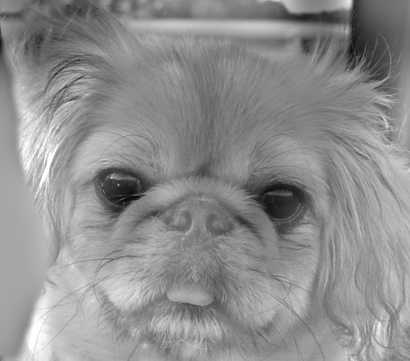
\includegraphics[width=\textwidth]{images/Hybrid_Swapped_Set1.jpg}
        \caption{مجموعه اول (نزدیک: سگ، دور: گربه)}
    \end{subfigure}
    \hfill
    \begin{subfigure}{0.5\textwidth}
        \centering
        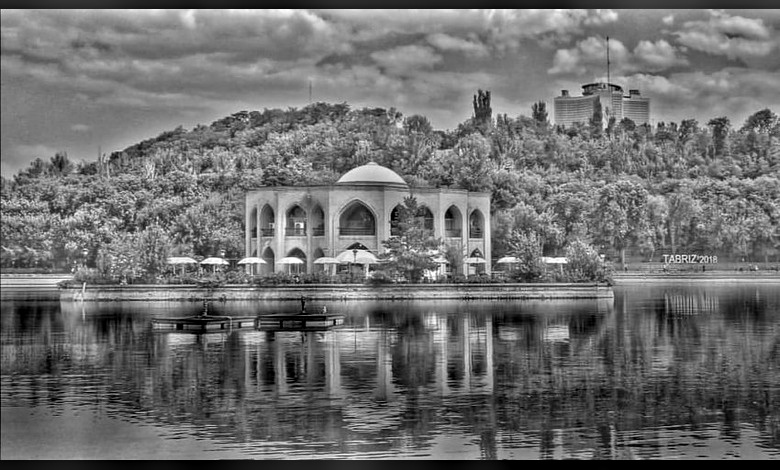
\includegraphics[width=\textwidth]{images/Hybrid_Swapped_Set2.jpg}
        \caption{مجموعه دوم (نزدیک: منظره، دور: پل)}
    \end{subfigure}
    \caption{تصاویر هیبریدی تولید شده پس از جابجایی نقش فرکانسی تصاویر}
    \label{fig:swapped_hybrid}
\end{figure}